\section{Problem 3: Momentum Shift Predictor Based on MM-LSTM}

\subsection{Model Structure of the Momentum Shift Predictor}\label{sec:swing_predict_model}
Based on the MM-LSTM model in Section \ref{sec:momentum_lstm}, we formulate a time-series model of the change in player scores that predicts when the situation in a match shifts from favoring one player to favoring another based on its gradient. The formula for our model is as follows:

% 描述了斜率相对差公式与动量的关系
\begin{equation}
     {K_{relative}}{(n, m)} = \frac{1}{n-m} \cdot \sum_{i=m+1}^{n} [P_i + 0.5] = \frac{1}{n-m} \cdot \sum_{i=m+1}^{n} [A+\alpha (p) + 0.5]
\end{equation}


Firstly, let's consider the score situation between two athletes, both gradually increasing over time. We assume that the functions describing these two evolving conditions are denoted as \(f_{1}\) and \(f_{2}\). Therefore, we can establish a simple mapping relationship as follows:
\begin{equation}
\left\{
\begin{aligned}
    y_{1} &= f_{1}(t) \\
    y_{2} &= f_{2}(t)
\end{aligned}
\right.
\end{equation}

In this case, we take the difference between the scores of the two athletes:
\begin{equation}
    y_1 - y_2  =  f_{1}(t) -  f_{2}(t)
\end{equation}

The gradient of their score function curves can be expressed as:
\begin{equation}
\left\{
\begin{aligned}
    % k_1 &= \frac{\delta y_{1}}{\delta t}  \\
    % k_2 &= \frac{\delta y_{2}}{\delta t}
    k_1 &= \frac{\delta y_{1}}{\delta t}  \\
    k_2 &= \frac{\delta y_{2}}{\delta t}
\end{aligned}
\right.
\end{equation}

At this point, based on our difference in scores, we can obtain a difference function whose gradient can be expressed as:
\begin{equation}
\label{ss}
    {K_{relative}}{(n, m)} = \frac{\delta (y_n - y_m)}{\delta t} = 
    \frac{\delta y_n}{\delta t} -   \frac{\delta y_m}{\delta t}
    = k_n - k_m
\end{equation}

And since the score for the nth round is determined based on the score from the (n-1)th round, the decision to score in each round relies on approximating the probability obtained from the MM-LSTM model. The probability results are rounded to obtain a binary outcome, indicating either victory (1) or failure (0). The scores are then updated based on this outcome, linking the MM-LSTM probability model with the scoring function. In another perspective, this can be viewed as a recursive formula. On this basis, we can also derive a scoring probability formula over a certain period:
\begin{equation}
    y_n = y_{n-1} + [P_n+0.5] \Longrightarrow
    y_n = y_m + \sum_{i=m+1}^{n} [P_i + 0.5] 
\end{equation}

The preceding formulas have successfully established a unified connection between probability and scores. Moving forward, let's further explore the relationship between momentum and gradient.

The following formula describes the relationship between the formula for relative gradient difference and momentum. The relative gradient difference is a metric (refer to Formula \ref{ss}) indicating score changes relative to time (or points). Here, n-m represents the variation in scores over a time period of n-m. In general, we typically set n-m to 3 (as we opted for interpolation rather than fitting). In this scenario, the score difference during this period reflects the variation in scores – the cumulative sum of whether each match results in a score. The probability P, predicted by the MM-LSTM model, approximates whether each match results in a score. Rounding P yields a binary outcome: victory (1) or failure (0). In the case of victory, points are added, causing the gradient to increase; in the event of failure, no points are added, maintaining the gradient. (Considering the relatively modest quantity of gradient, i.e., the increment in victories, over short time periods, plotting a graph with large swings may not be conducive for observation, hence the choice of a relatively large yet manageable value of 3.)

Moreover, in light of Formula \ref{ll}, where we interpret probability as momentum, we have intricately linked the relative gradient difference to momentum. Consequently, the relative gradient difference has become a key metric for analyzing changes in momentum.
\begin{equation}
\label{eq:formula25}
K_{relative}{(n, m)} = \frac{1}{n-m} \cdot \sum_{i=m+1}^{n} [P_i + 0.5] = \frac{1}{n-m} \cdot \sum_{i=m+1}^{n} [A+\alpha (p) + 0.5]
\end{equation}

The following formula represents the count of correct predictions, where \(P_i\) denotes the probability predicted at position i, representing the success probability for play 1. Applying the nested rounding function, when the prediction is successful (victory), it is rounded to 0, and when it fails (loss), it is rounded to 1. Adding 1 is done to convert the dimensional indicator of successful predictions to correspond with the dimensional indicator of \(point\_victor\). This allows for the assessment of the number of incorrect predictions. Substituting this into the frequency formula reflects the probability situation:

\begin{equation}
\label{eq:formula26}
N_{false}=\sum_{i=1}^{n}|1+[P_{i}+0.5]-Point\_victor_i|\end{equation}

The following formula is an inductive formula for calculating the final prediction accuracy:

\begin{equation}
\label{eq:formula27}
\eta_{accuracy}=\frac{N_{true}}{N_{total}}=\frac{N_{true}}{N_{true}+N_{false}} = 1-\frac{N_{false}}{N_{total}}
\end{equation}

\subsection{Factor Contribution Analysis}\label{sec:factor_contribution}
To test which factors contributed most to the model, we used a gradient importance analysis. The gradient represents the direction in which the function grows fastest at a given point, and its magnitude quantifies this maximum growth rate. For the model built in Section \ref{sec:swing_predict_model}, we calculated the partial derivative of each input with respect to the output, and then calculated the absolute value of that partial derivative and normalized it. The final normalized value obtained represents the degree of contribution of the inputs to the output.The contribution degree of some of the input indicators is shown in Table \ref{tab:gradient_importance}.

% \begin{table}[htbp]
% \centering
% \begin{tabular}{ll|ll}
% \specialrule{.1em}{0em}{0em} % 添加粗分割线
% \textbf{Factor Name} & \textbf{Value} & \textbf{Factor Name} & \textbf{Value} \\
% \specialrule{.1em}{0em}{0em} % 添加粗分割线
% point\_no & 0.0026 & serve\_no & 0.0305\\
% speed\_mph & 0.0007& game\_victor & 0.0369 \\ 
% rally\_count & 0.0319&set\_victor & 0.0282   \\ 
% server & 0.0729 & serve\_width & 0.0018 \\ 
% serve\_depth & 0.0247 & return\_depth & 0.0212 \\
% p1\_sets & 0.0196 & p2\_sets & 0.1217\\ 
% p1\_games & 0.0016 & p2\_games & 0.0061 \\ 
% p1\_points\_won & 0.0201 & p2\_points\_won & 0.0183\\ 
% p1\_ace & 0.0145 & p2\_ace & 0.0956\\ 
% p1\_winner & 0.0711 & p2\_winner & 0.0272\\ 
% p1\_double\_fault & 0.0055 & 
% p2\_double\_fault & 0.0141 \\ p1\_unf\_err & 0.0598 & 
% p2\_unf\_err & 0.1016 \\ p1\_net\_pt & 0.0761 & 
% p2\_net\_pt & 0.0884 \\ p1\_distance\_run & 0.0061 &
% p2\_distance\_run & 0.0011 \\ 
% \specialrule{.1em}{0em}{0em} % 添加粗分割线
% \end{tabular}
% \caption{Gradient importance analysis}
% \label{tab:gradient_importance}
% \end{table}

% \begin{table}[htbp]
% \centering
% \begin{tabular}{ll|ll}
% \specialrule{.1em}{0em}{0em} % 添加粗分割线
% \textbf{Factor} & \textbf{Value} & \textbf{Factor} & \textbf{Value} \\ 
% \specialrule{.1em}{0em}{0em} % 添加粗分割线
% point\_no & 0.0117 & p1\_double\_fault & 0.0283 \\
% server & 0.0100 & p2\_double\_fault & 0.0203 \\
% serve\_no & 0.0107 & p1\_unf\_err & 0.1662 \\
% p1\_points\_won & 0.0003 & p2\_unf\_err & 0.1894 \\
% p2\_points\_won & 0.0179 & p1\_net\_pt & 0.0085 \\
% p1\_ace & 0.0135 & p2\_net\_pt & 0.1064 \\
% p2\_ace & 0.0101 & p1\_distance\_run & 0.0068 \\
% p1\_winner & 0.1415 & p2\_distance\_run & 0.0065 \\
% p2\_winner & 0.1223 & rally\_count & 0.0129 \\
% p1\_double\_fault & 0.0283 & speed\_mph & 0.0029 \\
% p2\_double\_fault & 0.0203 & serve\_width & 0.0666 \\
% p1\_unf\_err & 0.1662 & serve\_depth & 0.0085 \\
% p2\_unf\_err & 0.1894 & return\_depth & 0.0386 \\ 
% \specialrule{.1em}{0em}{0em} % 添加粗分割线
% \end{tabular}
% \caption{Gradient importance analysis}
% \label{tab:gradient_importance}
% \end{table}

% \begin{table}[htbp]
% \centering
% \begin{tabular}{@{}ll|ll@{}}
% \specialrule{.1em}{0em}{0em} % 添加粗分割线
% \textbf{Factor} & \textbf{Value} & \textbf{Factor} & \textbf{Value} \\ 
% \specialrule{.1em}{0em}{0em} % 添加粗分割线
% point\_no & 0.0117 & p1\_double\_fault & 0.0283 \\
% server & 0.0100 & p2\_double\_fault & 0.0203 \\
% serve\_no & 0.0107 & p1\_unf\_err & 0.1662 \\
% p1\_points\_won & 0.0003 & p2\_unf\_err & 0.1894 \\
% p2\_points\_won & 0.0179 & p1\_net\_pt & 0.0085 \\
% p1\_ace & 0.0135 & p2\_net\_pt & 0.1064 \\
% p2\_ace & 0.0101 & p1\_distance\_run & 0.0068 \\
% % p1\_winner & 0.1415 & p2\_distance\_run & 0.0065 \\
% % p2\_winner & 0.1223 & rally\_count & 0.0129 \\
% % p1\_double\_fault & 0.0283 & speed\_mph & 0.0029 \\
% % p2\_double\_fault & 0.0203 & serve\_width & 0.0666 \\
% % p1\_unf\_err & 0.1662 & serve\_depth & 0.0085 \\
% % p2\_unf\_err & 0.1894 & return\_depth & 0.0386 \\ 
% \specialrule{.1em}{0em}{0em} % 添加粗分割线
% \end{tabular}
% \caption{Gradient importance analysis}
% \label{tab:gradient_importance}
% \end{table}

% \begin{table}[htbp]
% \centering
% \begin{tabular}{@{}ll|ll|ll|ll@{}}
% \specialrule{.1em}{0em}{0em} % 添加粗分割线
% \textbf{Factor} & \textbf{Value} & \textbf{Factor} & \textbf{Value} & \textbf{Factor} & \textbf{Value} & \textbf{Factor} & \textbf{Value} \\ 
% \specialrule{.1em}{0em}{0em} % 添加粗分割线
% point\_no & 0.0117 & p1\_double\_fault & 0.0283 & p1\_winner & 0.1415 & p2\_distance\_run & 0.0065 \\
% server & 0.0100 & p2\_double\_fault & 0.0203 & p2\_winner & 0.1223 & rally\_count & 0.0129 \\
% serve\_no & 0.0107 & p1\_unf\_err & 0.1662 & p1\_double\_fault & 0.0283 & speed\_mph & 0.0029 \\
% p1\_points\_won & 0.0003 & p2\_unf\_err & 0.1894 & p2\_double\_fault & 0.0203 & serve\_width & 0.0666 \\
% p2\_points\_won & 0.0179 & p1\_net\_pt & 0.0085 & p1\_unf\_err & 0.1662 & serve\_depth & 0.0085serve \\
% p1\_ace & 0.0135 & p2\_net\_pt & 0.1064 & p2\_unf\_err & 0.1894 & return\_depth & 0.0386 \\
% p2\_ace & 0.0101 & p1\_distance\_run & 0.0068 & & & & \\
% \specialrule{.1em}{0em}{0em} % 添加粗分割线
% \end{tabular}
% \caption{Gradient importance analysis}
% \label{tab:gradient_importance}
% \end{table}

\begin{table}[htbp]
\centering
\caption{Gradient Importance Analysis}
\vspace{8pt}
\begin{tabular}{@{}ll|ll|ll@{}}
\specialrule{.1em}{0em}{0em} % 添加粗分割线
\textbf{Factor} & \textbf{Value} & \textbf{Factor} & \textbf{Value} & \textbf{Factor} & \textbf{Value} \\ 
\specialrule{.1em}{0em}{0em} % 添加粗分割线
point\_no & 0.0117 & p1\_double\_fault & 0.0283 & p1\_winner & 0.1415 \\
server & 0.0100 & p2\_double\_fault & 0.0203 & p2\_winner & 0.1223 \\
serve\_no & 0.0107 & p1\_unf\_err & 0.1662 & p1\_double\_fault & 0.0283 \\
serve\_width & 0.0666 & p2\_unf\_err & 0.1894 & p2\_double\_fault & 0.0203 \\
return\_depth & 0.0386 & p1\_net\_pt & 0.0085 & p1\_unf\_err & 0.1662 \\
p1\_ace & 0.0135 & p2\_net\_pt & 0.1064 & p2\_unf\_err & 0.1894 \\
\specialrule{.1em}{0em}{0em} % 添加粗分割线
\end{tabular}
% \caption{Gradient importance analysis}
\label{tab:gradient_importance}
\end{table}

% \begin{table}[htbp]
% \centering
% \begin{tabular}{@{}ll|ll|ll@{}}
% \specialrule{.1em}{0em}{0em} % 添加粗分割线
% \textbf{Factor} & \textbf{Value} & \textbf{Factor} & \textbf{Value} & \textbf{Factor} & \textbf{Value} \\ 
% \specialrule{.1em}{0em}{0em} % 添加粗分割线
% point\_no & 0.0117 & p1\_double\_fault & 0.0283 & p1\_winner & 0.1415 \\
% server & 0.0100 & p2\_double\_fault & 0.0203 & p2\_winner & 0.1223 \\
% serve\_no & 0.0107 & p1\_unf\_err & 0.1662 & serve\_width & 0.0666 \\
% p2\_points\_won & 0.0179 & p2\_unf\_err & 0.1894 & serve\_depth & 0.0085 \\
% p1\_ace & 0.0135 & p1\_net\_pt & 0.0085 & return\_depth & 0.0386 \\
% p2\_ace & 0.0101 & p2\_net\_pt & 0.1064 & \\
% \specialrule{.1em}{0em}{0em} % 添加粗分割线
% \end{tabular}
% \caption{Gradient importance analysis}
% \label{tab:gradient_importance}
% \end{table}



From the table, we can see that p2\_unf\_err contributes the most to the output with 0.1894, p1\_unf\_err contributes the second most to the output with 0.1662, and the rest of the metrics with top 8 contributions are: p\_1winner, p2\_winner, p2\_net\_pt, serve\_width, return\_depth, p1\_double\_fault. we visualized these data as Figure \ref{fig:gradients_pie}.


% We extracted 8 factors with the largest contributions and visualized their contributions at Figure \ref{fig:gradients_pie}

\begin{figure}[htbp]
    \centering
    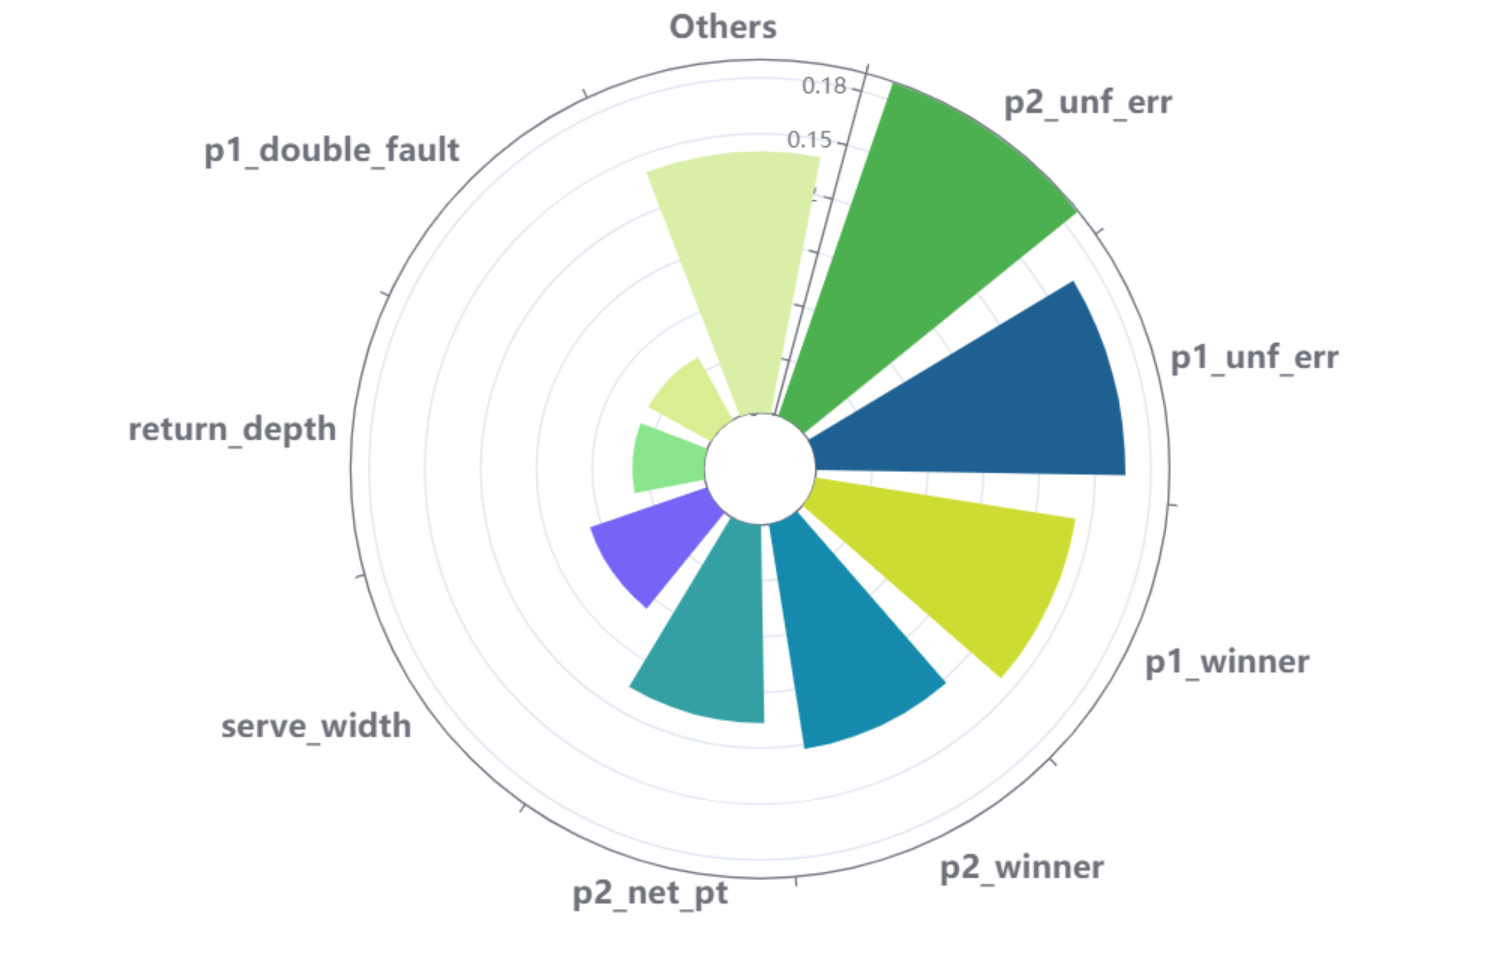
\includegraphics[width=0.8\textwidth]{figure/bar-polar-label-radial.png}
    % \vspace{-0.3cm}
    \caption{ Factors\textquotesingle~Contribution Based on Gradient Importance Analysis
    \textnormal{}}
    \label{fig:gradients_pie}
    % \vspace{-0.5cm}
\end{figure}

\subsection{Match recommendations based on momentum changes}

Here, we first analyze the quantification of momentum. Regarding the relative strength factors in this model, they are known quantities that allow us to assess the player's strength by comparing their historical performances with other players. Simultaneously, we can extract data from the opponent's match records, such as the timing and proportion of serving faults as the first server, as well as the increase in the number of points won over time. This information helps us understand when the player is more active and demonstrates stronger abilities during the match.

The MM-LSTM model provides the swing in the probability of winning from the beginning to the end, offering insights into the player's changing momentum. Here, the factors unrelated to the match time are analogized as "m", while those related to the match time are analogized as "v". The momentum "p" is influenced by changes in "m" of the same units, causing changes in "v" and directly affecting changes in "p". Therefore, both factors need to be considered in assessing the player's performance.

\begin{figure}[htbp]
    \centering
    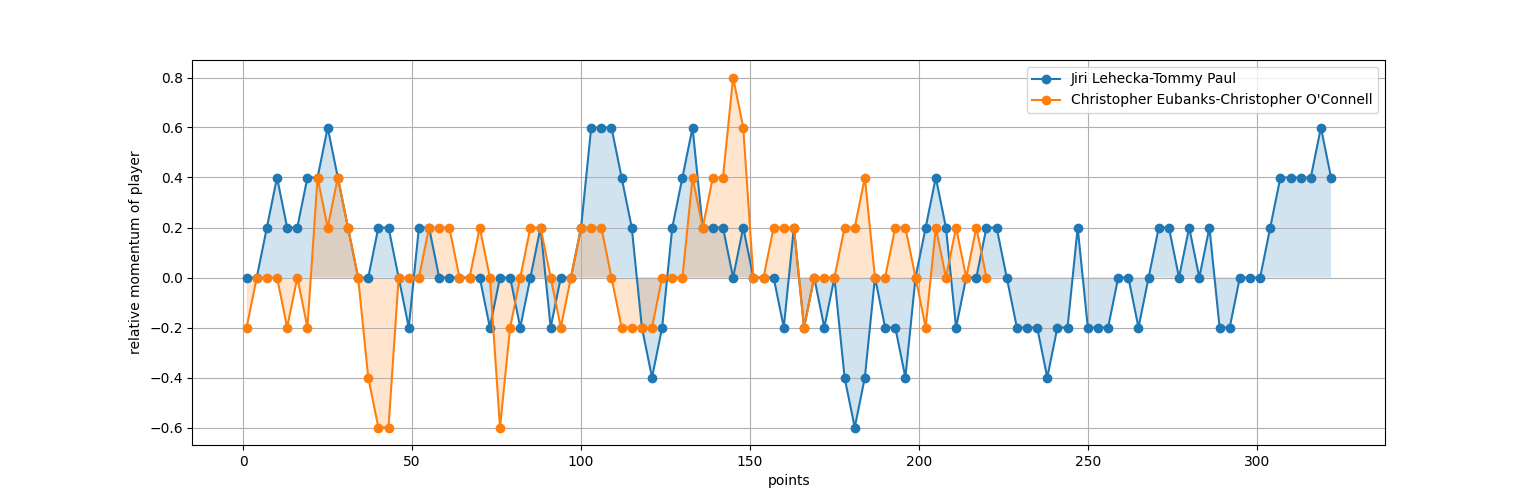
\includegraphics[width=1.1\textwidth]{figure/p_3_2_1.png}
    % \vspace{-0.3cm}
    \caption{The Momentum Indicator Changes in Two Matches
    \textnormal{}}
    % \label{fig:gradients_pie}
    % \vspace{-0.5cm}
\end{figure}



The figure above displays the relative momentum changes between the two players in two separate matches, with 0 as the starting point. It is evident that the trend of relative momentum changes is unpredictable. For instance, in the match represented by the blue line, Jini initially had the advantage but later allowed the opponent to come from behind. This swing is also reflected in the scoring situation.

Based on the correlation analysis between momentum and other factors, the following recommendations can be derived:



Psychological Considerations:
\begin{itemize}[label=\textbf{\normalsize$\bullet$}]
    \item As the saying goes, "make the best effort in the first push, weaken in the second, and exhaust in the third", it can be fair to conclude that, except for the first set, serving has no impact on winning that set.\cite{p321} For the first set, serving opportunities should be seized, and caution should be exercised when facing the opponent's serve. Do not become overconfident or careless due to an early advantage, as it may lead to failure in subsequent matches.
    \item Maintaining composure is crucial when facing uncontrollable outcomes with decisive consequences. The player's mentality directly determines the strength of their current momentum in the game. Unstoppable winning serves and unforced errors can be decisive, with a \(100\%\) impact on the outcome of the current exchange. Players should maintain a stable mindset, as the probability of such serves is very small, around \(5\%\), and subject to uncertainty over time. Therefore, there's no need to overly focus on such situations; learn to keep your composure. Additionally, after an unstoppable serve, the calculated probability of winning in the next five games increases to \(60\%\), highlighting the significant role of decisive factors in determining momentum.
    \item Stay humble and composed. In the data, when the current score is in favor of the player, the average probability of winning the point is \(26.81\%\), indicating that a lead may likely lead to failure. Be cautious in facing break points; winners facing break points tend to score more points, while losers struggle to maintain their level. Breaking and then holding serve is often more challenging than sailing smoothly with the wind.\cite{p322}
\end{itemize}

\begin{figure}[htbp]
    \centering
    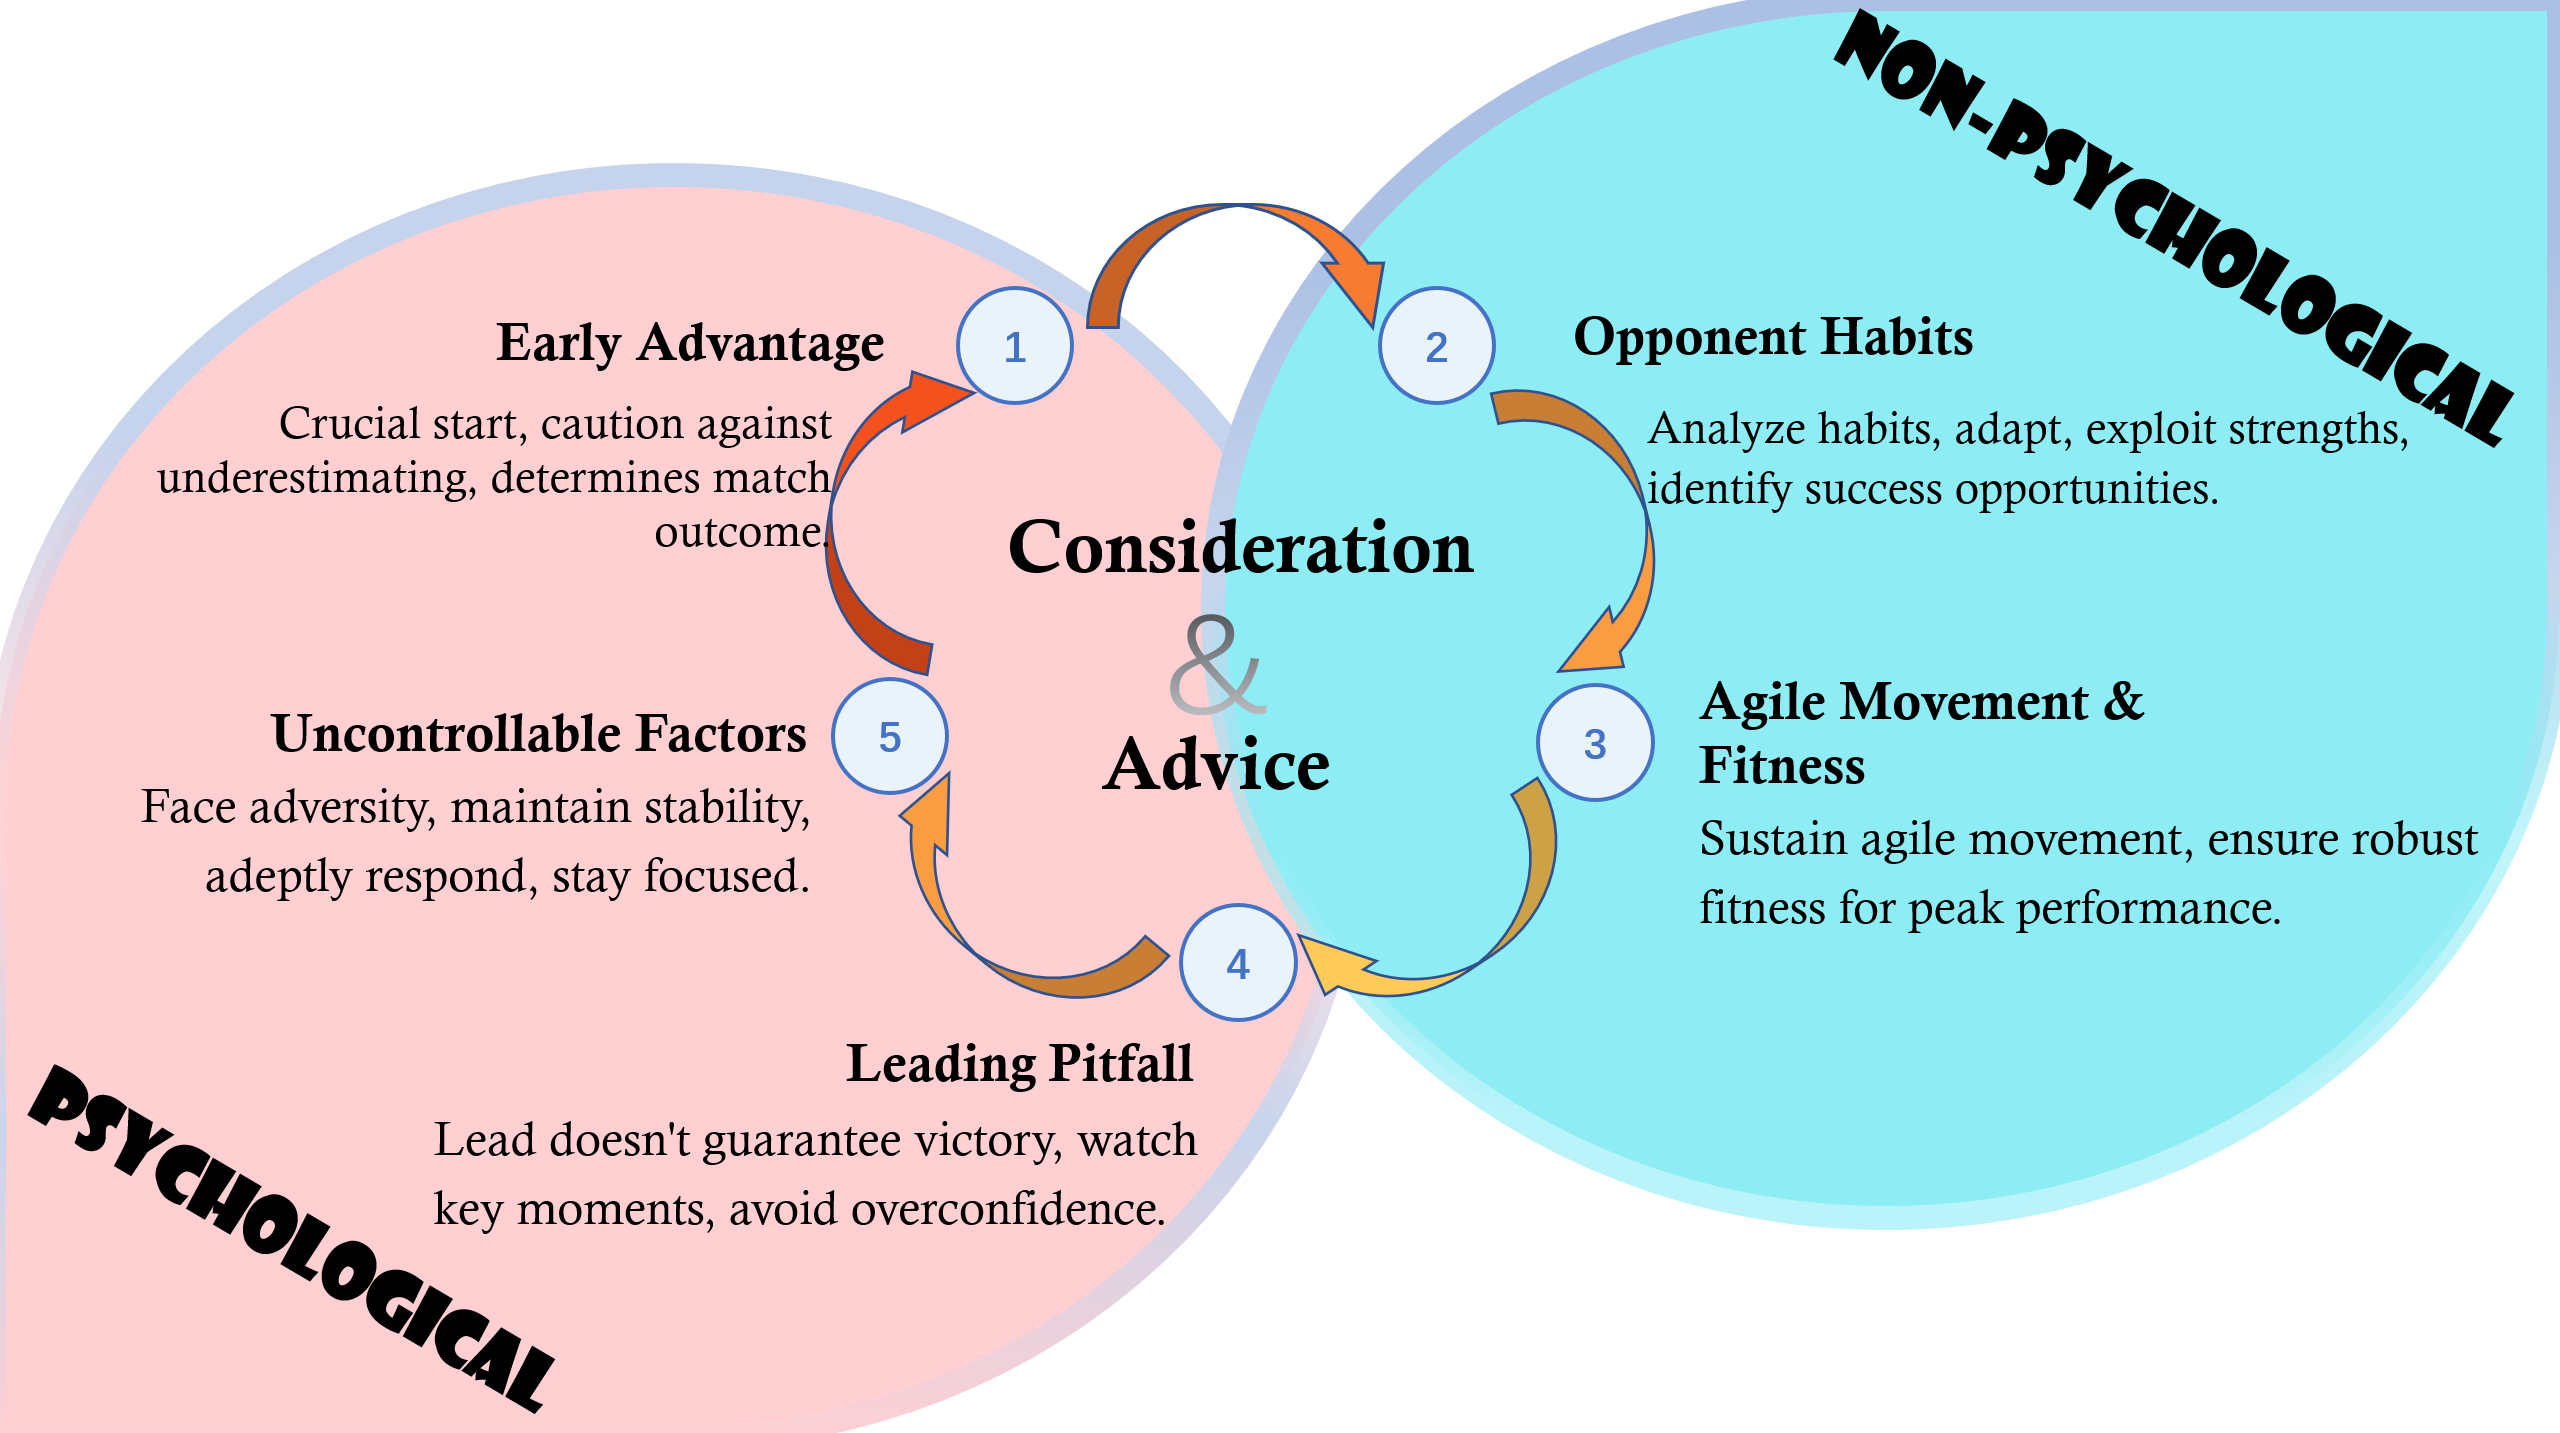
\includegraphics[width=0.95\textwidth]{figure/memo.png}
    % \vspace{-0.3cm}
    \caption{Suggestions for Athletes
    \textnormal{}}
    % \label{fig:gradients_pie}
    % \vspace{-0.5cm}
\end{figure}

Non-psychological Considerations:
\begin{itemize}[label=\textbf{\normalsize$\bullet$}]

\item Maintain flexibility on the court and avoid being confined to a specific area. According to data analysis, if a player is positioned at the net, their probability of scoring is \(69.88\%\), indicating a significant advantage in playing at the net. Additionally, when calculating the win rate with a running distance exceeding the average, it is \(48.75\%\), slightly lower than the average. This could be attributed to the physical exhaustion caused by increased running distance. However, in the statistics, it was found that the running distance in victorious matches tends to be slightly above the average. This suggests that while physical exhaustion has a minimal impact on victory, agile positioning and an active physique play a crucial role.

\item Carefully study the opponent's past match videos and data, paying attention to their strengths and weaknesses. Understand the opponent's playing style to formulate better tactics, including their preference for forehand or backhand, hitting power, speed, running distance, etc. According to the data, most players tend to prefer serving in the "w" direction, particularly favoring "CTL" near the sidelines, and their return shots usually have considerable depth. However, this is a general statistical observation for all players, and individual analysis should be conducted for specific opponents based on their historical data.
\end{itemize}

In conclusion, we believe that the most crucial aspect is to learn to control your own momentum. The main reason for the swings in momentum fundamentally depends on the changes in a player's strength over time on the court. By mastering and controlling these changes, you can achieve autonomy and make your momentum appear random while being controlled by yourself. This allows for the use of deceptive tactics to mislead opponents or to make continuous and aggressive progress, aiming for a decisive victory.





